\documentclass[ignorenonframetext,]{beamer}
\setbeamertemplate{caption}[numbered]
\setbeamertemplate{caption label separator}{: }
\setbeamercolor{caption name}{fg=normal text.fg}
\beamertemplatenavigationsymbolsempty
\usepackage{lmodern}
\usepackage{amssymb,amsmath}
\usepackage{ifxetex,ifluatex}
\usepackage{fixltx2e} % provides \textsubscript
\ifnum 0\ifxetex 1\fi\ifluatex 1\fi=0 % if pdftex
  \usepackage[T1]{fontenc}
  \usepackage[utf8]{inputenc}
\else % if luatex or xelatex
  \ifxetex
    \usepackage{mathspec}
  \else
    \usepackage{fontspec}
  \fi
  \defaultfontfeatures{Ligatures=TeX,Scale=MatchLowercase}
\fi
\usetheme[]{Madrid}
\usecolortheme{seahorse}
\usefonttheme{serif}
% use upquote if available, for straight quotes in verbatim environments
\IfFileExists{upquote.sty}{\usepackage{upquote}}{}
% use microtype if available
\IfFileExists{microtype.sty}{%
\usepackage{microtype}
\UseMicrotypeSet[protrusion]{basicmath} % disable protrusion for tt fonts
}{}
\newif\ifbibliography
\usepackage{natbib}
\bibliographystyle{plainnat}
\hypersetup{
            pdftitle={PhD Midway Seminar},
            pdfauthor={Raju Rimal},
            pdfborder={0 0 0},
            breaklinks=true}
\usepackage{longtable,booktabs}
\usepackage{caption}
% These lines are needed to make table captions work with longtable:
\makeatletter
\def\fnum@table{\tablename~\thetable}
\makeatother

% Prevent slide breaks in the middle of a paragraph:
\widowpenalties 1 10000
\raggedbottom

\AtBeginPart{
  \let\insertpartnumber\relax
  \let\partname\relax
  \frame{\partpage}
}
\AtBeginSection{
  \ifbibliography
  \else
    \let\insertsectionnumber\relax
    \let\sectionname\relax
    \frame{\sectionpage}
  \fi
}
\AtBeginSubsection{
  \let\insertsubsectionnumber\relax
  \let\subsectionname\relax
  \frame{\subsectionpage}
}

\setlength{\parindent}{0pt}
\setlength{\parskip}{6pt plus 2pt minus 1pt}
\setlength{\emergencystretch}{3em}  % prevent overfull lines
\providecommand{\tightlist}{%
  \setlength{\itemsep}{0pt}\setlength{\parskip}{0pt}}
\setcounter{secnumdepth}{0}
\usepackage{textpos}
\usepackage{mathpazo}

\definecolor{first}{HTML}{009D7F}
\definecolor{first-text}{HTML}{F2F2F2}
\definecolor{second}{HTML}{00997D}
\definecolor{second-text}{HTML}{FDFDFD}
\definecolor{third}{HTML}{008068}
\definecolor{third-text}{HTML}{FFFFFF}
\setbeamercolor*{palette primary}{use=structure,fg=first-text,bg=first}
\setbeamercolor*{palette secondary}{use=structure,fg=second-text,bg=second}
\setbeamercolor*{palette tertiary}{use=structure,fg=third-text,bg=third}
\setbeamercolor{item projected}{fg=white,bg=third}

\addtobeamertemplate{frametitle}{}{%
\begin{textblock*}{100mm}(0.92\textwidth,-0.85cm)

\includegraphics[height=0.75cm]{images/LogoNMBUwhite}
\end{textblock*}}

\titlegraphic{
\includegraphics[height=1cm]{images/LogoNMBU}}
% \renewcommand*{\bibfont}{\scriptsize}

\makeatletter
\setbeamertemplate{footline}
{
  \leavevmode%
  \hbox{%
  \begin{beamercolorbox}[wd=.15\paperwidth,ht=2.25ex,dp=1ex,center]{author in head/foot}%
    \usebeamerfont{author in head/foot}\insertshortauthor
  \end{beamercolorbox}%
  \begin{beamercolorbox}[wd=.6\paperwidth,ht=2.25ex,dp=1ex,center]{title in head/foot}%
    \usebeamerfont{title in head/foot}\inserttitle
  \end{beamercolorbox}%
  \begin{beamercolorbox}[wd=.25\paperwidth,ht=2.25ex,dp=1ex,right]{date in head/foot}%
    \usebeamerfont{date in head/foot}\insertshortdate{}\hspace*{2em}
    \insertframenumber{} / \inserttotalframenumber\hspace*{2ex} 
  \end{beamercolorbox}}%
  \vskip0pt%
}
\makeatother

\title{PhD Midway Seminar}
\subtitle{Simulation Tool and its application}
\author{Raju Rimal}
\institute{\textbf{Supervisors}\\
Solve Sæbø, Tryge Almøy}
\date{02 March, 2017}

\begin{document}
\frame{\titlepage}

\section{Introduction}\label{introduction}

\begin{frame}{My PhD Plan}

\hypertarget{left}{}

\hypertarget{right}{}
\begin{itemize}[<+->]
\tightlist
\item
  Make {Simulation Tools} for multi-response linear model data
\item
  Using the tool, compare various {estimation techniques} and
  {understand} them
\item
  {Extend} the simulation tool incorporating model with {background
  information}
\item
  Apply this extended tool to {test multi-matrix extension of PLS}
  models such as LPLS and UPLS
\end{itemize}

\end{frame}

\begin{frame}{What I learn}

\begin{itemize}[<+->]
\tightlist
\item
  Advanced Multivariate Model and technique to analyze it
\item
  Programming concept for developing statistical packages and
  applications for various statistical methods
\item
  Extending and improving existing methods in statistics
\item
  And, Obviously, to properly document what I have done
\end{itemize}

\end{frame}

\begin{frame}[fragile]{Today's Special}

Today I will talk about:

\begin{itemize}[<+->]
\tightlist
\item
  Simulation tool ({\texttt{simulatr}}) we are building
\item
  A {competative study} of various estimation techniques by simulating
  linear model data using \texttt{simulatr}
\end{itemize}

\end{frame}

\section{\texorpdfstring{\texttt{simrel-m}: A versatile tool for
simulating multi-response linear model
data}{simrel-m: A versatile tool for simulating multi-response linear model data}}\label{simrel-m-a-versatile-tool-for-simulating-multi-response-linear-model-data}

\begin{frame}[fragile]{Overview}

\begin{itemize}[<+->]
\tightlist
\item
  An extension of \texttt{simrel} \citep{saebo2015simrel} r-package
\item
  Uses the idea of reduction of random regression model by separating
  latent space of \(\mathbf{X}\) into subspaces that is relevant and
  irrelevant for predicting each response
\item
  The underlying concept is based on reparameterizing the population
  model, \[
  \mathbf{Y} = \boldsymbol{\mu}_{Y} + \mathbf{B}^t\left(\mathbf{X} - \boldsymbol{\mu}_X\right) + \boldsymbol{\epsilon}
  \] where,
  \(\boldsymbol{\epsilon} \sim N(0, \boldsymbol{\Sigma}_{Y|X})\)
\end{itemize}

\end{frame}

\begin{frame}{Underlying procedure}

\hypertarget{left}{}

\hypertarget{right}{}
\begin{itemize}[<+->]
\tightlist
\item
  Collect population input parameter from users such as: number of
  variables, coefficient of determination and the position of relevant
  components
\item
  Make a covariance matrix satisfying input parameters
\item
  Rotate the covariance matrix orthogonally
\item
  Sample calibration and validation sets
\end{itemize}

\end{frame}

\section{A comparative study of different estimation methods using
simulated
data}\label{a-comparative-study-of-different-estimation-methods-using-simulated-data}

\begin{frame}[fragile]{Overview}

\begin{block}{Four estimtion methods were considered}

\hypertarget{left}{}
\subsubsection{Ordinary Least Squares}\label{ordinary-least-squares}

\begin{itemize}
\tightlist
\item
  Although unbiased, suffer highly from multicollinearity
\item
  Widely used and can be used as reference for comparison
\end{itemize}

\subsubsection{Envelope}\label{envelope}

\begin{itemize}
\tightlist
\item
  Based on Maximum Likelihood but works better than OLS in \(p\)
  approaches \(n\)
\item
  Our analysis is based on envelope of predictor or \texttt{xenvelope}
\end{itemize}

\hypertarget{right}{}
\subsubsection{Partial Least Squares}\label{partial-least-squares}

\begin{itemize}
\tightlist
\item
  Well established and widely used method
\item
  Based on Latent Structure and free of multicollinearity problem
\end{itemize}

\subsubsection{Bayes PLS}\label{bayes-pls}

\begin{itemize}
\tightlist
\item
  Bayesian Estimation of regression coefficient
\item
  Promising performance was shown in previous studies
  \citep{helland2012near}
\end{itemize}

\end{block}

\end{frame}

\begin{frame}{Simulation Design}

From the possible combination of following parameter combination, 32
calibration sets were simulated with 5 replication of each.

\begin{longtable}[]{@{}rrrrr@{}}
\toprule
Number of sample observation & 50 & 50 & 50 & 50\tabularnewline
Number of predictor variables & 15 & 40 & 15 & 40\tabularnewline
Coefficient of determination & 0.5 & 0.9 & 0.5 & 0.9\tabularnewline
Position of relevant component & 1, 2 & 1, 3 & 2, 3 & 1, 2,
3\tabularnewline
Decaying factor of eigenvalues & 0.5 & 0.9 & 0.5 & 0.9\tabularnewline
\bottomrule
\end{longtable}

\end{frame}

\begin{frame}{A Systematic Comparison}

\end{frame}

\section{Conclusion}\label{conclusion}

\begin{frame}{Simulation Design}

grow

shrink

fade-out

fade-up (also down, left and right!)

visible only once

blue only once

highlight-red

highlight-green

highlight-blue

\end{frame}

\begin{frame}{Simulatr App}

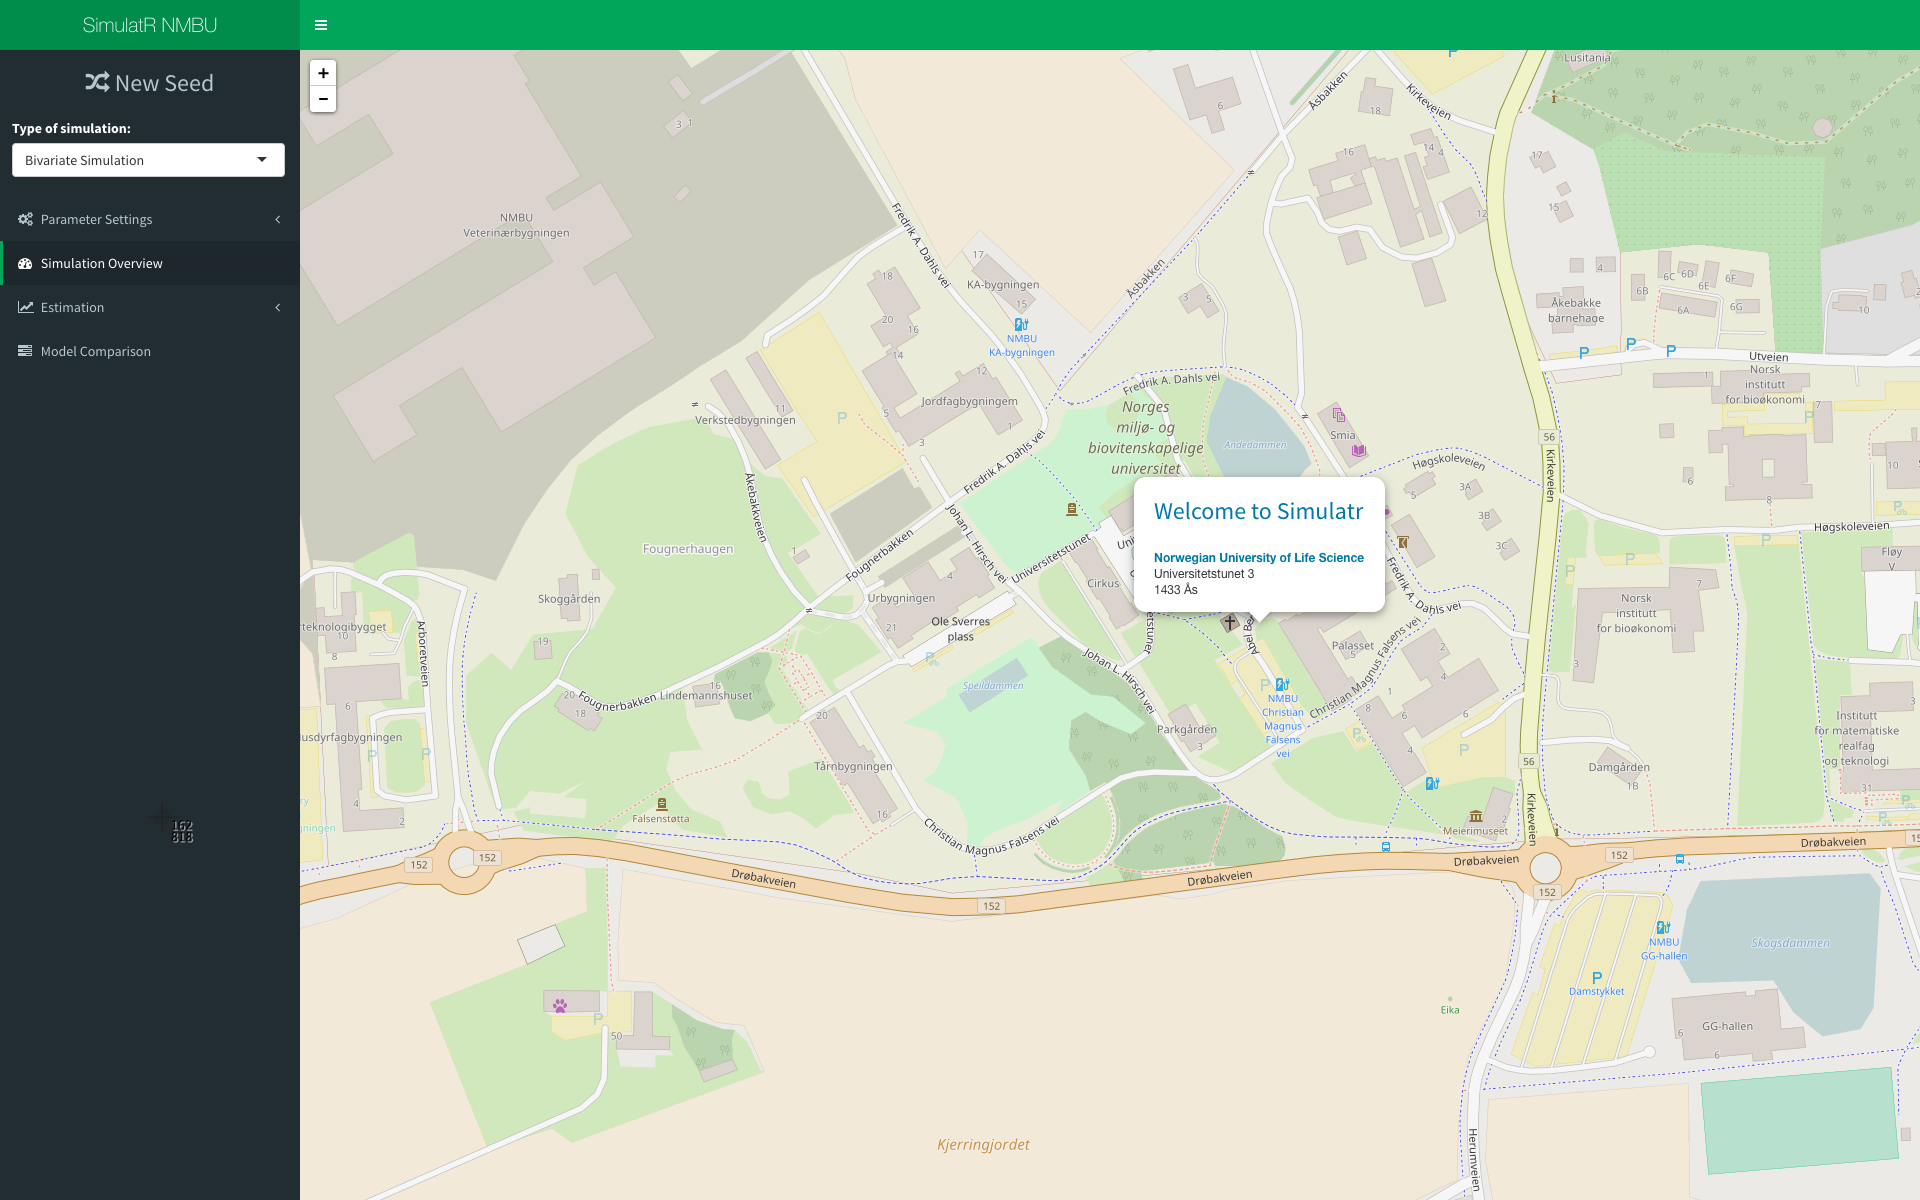
\includegraphics[width=0.8\linewidth]{images/simulatr-screenshot}

\end{frame}

\section{}\label{section}

\section{References}\label{references}

\begin{frame}{References}

\end{frame}

\begin{frame}[allowframebreaks]{}
\bibliographytrue
\bibliography{references.bib}
\end{frame}

\end{document}
